\documentclass[11pt]{article}
\usepackage[a4paper, margin=1in, headheight=13.6pt]{geometry}
\usepackage[utf8]{inputenc}
\usepackage{titlesec}
\usepackage{enumitem}
\usepackage{listings}
\usepackage{xcolor}
\usepackage{hyperref}
\usepackage{fancyhdr}
\usepackage{graphicx}
\usepackage{tabularx}
\usepackage{longtable}
\usepackage{booktabs}
\usepackage{multirow}
\usepackage{float}
\usepackage{imakeidx}
\usepackage{tcolorbox}

% Define colors for JSON syntax highlighting
\definecolor{jsonbackground}{rgb}{0.95,0.95,0.95}
\definecolor{jsonnumb}{rgb}{0.5,0.5,0.5}
\definecolor{jsonstr}{rgb}{0.6,0,0}
\definecolor{jsonpunct}{rgb}{0.5,0.5,0.5}
\definecolor{jsondelim}{rgb}{0.2,0.2,0.2}

% Define Dart language for listings
\lstdefinelanguage{Dart}{
  keywords={abstract, as, assert, async, await, break, case, catch, class, const, continue, covariant, default, deferred, do, dynamic, else, enum, export, extends, extension, external, factory, false, final, finally, for, Function, get, hide, if, implements, import, in, interface, is, library, mixin, new, null, on, operator, part, required, rethrow, return, set, show, static, super, switch, sync, this, throw, true, try, typedef, var, void, while, with, yield},
  sensitive=true,
  comment=[l]{//},
  morecomment=[s]{/*}{*/},
  morestring=[b]',
  morestring=[b]"
}

% Define YAML language for listings
\lstdefinelanguage{yaml}{
  keywords={true,false,null,yes,no},
  sensitive=false,
  comment=[l]{\#},
  morecomment=[s]{/*}{*/},
  morestring=[b]',
  morestring=[b]"
}

% Define JSON language for listings
\lstdefinelanguage{json}{
    basicstyle=\normalfont\ttfamily,
    numbers=left,
    numberstyle=\scriptsize,
    stepnumber=1,
    numbersep=8pt,
    showstringspaces=false,
    breaklines=true,
    frame=lines,
    backgroundcolor=\color{jsonbackground},
    literate=
     *{0}{{{\color{jsonnumb}0}}}{1}
      {1}{{{\color{jsonnumb}1}}}{1}
      {2}{{{\color{jsonnumb}2}}}{1}
      {3}{{{\color{jsonnumb}3}}}{1}
      {4}{{{\color{jsonnumb}4}}}{1}
      {5}{{{\color{jsonnumb}5}}}{1}
      {6}{{{\color{jsonnumb}6}}}{1}
      {7}{{{\color{jsonnumb}7}}}{1}
      {8}{{{\color{jsonnumb}8}}}{1}
      {9}{{{\color{jsonnumb}9}}}{1}
      {:}{{{\color{jsonpunct}{:}}}}{1}
      {,}{{{\color{jsonpunct}{,}}}}{1}
      {\{}{{{\color{jsondelim}{\{}}}}{1}
      {\}}{{{\color{jsondelim}{\}}}}}{1}
      {[}{{{\color{jsondelim}{[}}}}{1}
      {]}{{{\color{jsondelim}{]}}}}{1},
}

\makeindex[title={Index}, columns=2, intoc]

\pagestyle{fancy}
\fancyhf{}
\rhead{PhishSafe — Technical Documentation}
\lhead{Version 1.0}
\cfoot{\thepage}

\hypersetup{
    colorlinks=true,
    linkcolor=black,
    urlcolor=black,
    citecolor=blue,
    pdfborder={0 0 0}
}

\titleformat{\section}{\Large\bfseries\filcenter}{}{0em}{\underline}
\titleformat{\subsection}{\large\bfseries}{}{0em}{}
\titleformat{\subsubsection}{\normalsize\bfseries}{}{0em}{}

\definecolor{codegray}{rgb}{0.5,0.5,0.5}
\definecolor{backcolor}{rgb}{0.95,0.95,0.95}
\definecolor{deepblue}{rgb}{0,0,0.5}
\definecolor{deepred}{rgb}{0.6,0,0}
\definecolor{deepgreen}{rgb}{0,0.5,0}

\lstdefinestyle{mystyle}{
    backgroundcolor=\color{backcolor},
    commentstyle=\color{deepgreen},
    keywordstyle=\color{deepblue},
    numberstyle=\tiny\color{codegray},
    stringstyle=\color{deepred},
    basicstyle=\ttfamily\footnotesize,
    breakatwhitespace=false,
    breaklines=true,
    captionpos=b,
    keepspaces=true,
    numbers=left,
    numbersep=5pt,
    showspaces=false,
    showstringspaces=false,
    showtabs=false,
    tabsize=2,
    frame=single,
    rulecolor=\color{black!30}
}

\lstset{style=mystyle}

\tcbset{
  colback=gray!5,
  colframe=black!75,
  boxrule=0.8pt,
  arc=4pt,
  outer arc=4pt,
  fonttitle=\bfseries,
  coltitle=white,
  colbacktitle=black,
  title filled=true
}

\begin{document}

\vspace*{3cm}
\begin{center}
    {\Huge \textbf{PhishSafe SDK}}\\[1.2em]
    {\LARGE Technical Documentation}\\[1em]
    {\large Version 1.0}\\[0.5em]
    {\small Brought to you by team SudoCode}
\end{center}
\vfill

\newpage
\tableofcontents

\clearpage
\section{Introduction and Overview}

\subsection{Business Goals and Objectives}
PhishSafe SDK\index{PhishSafe SDK} is a behavioral authentication engine designed to detect post-login fraud and phishing threats in mobile applications through continuous behavioral tracking and trust scoring\index{trust scoring}. The system aims to:

\begin{itemize}
    \item Provide real-time fraud detection using behavioral biometrics\index{biometrics}
    \item Reduce account takeover incidents by 85\% within first year
    \item Maintain user privacy with on-device processing
    \item Integrate seamlessly with existing applications
    \item Provide actionable security insights through comprehensive dashboards
\end{itemize}

\subsection{Target Audience}
\begin{itemize}
    \item \textbf{Mobile App Users}: End-users who need protection against phishing\index{phishing protection}
    \item \textbf{Security Teams}: Fraud analysts and security professionals
    \item \textbf{Developers}: Mobile app developers integrating the SDK
    \item \textbf{Product Managers}: Stakeholders evaluating security solutions
\end{itemize}

\subsection{Core Functionality}
The PhishSafe SDK provides the following key features:

\begin{longtable}{|p{0.25\textwidth}|p{0.7\textwidth}|}
    \hline
    \textbf{Feature} & \textbf{Description} \\
    \hline
    Session Analytics\index{session analytics} & Monitors complete user session from login to logout \\
    \hline
    Location Tracking\index{location tracking} & Verifies geographical consistency during sessions \\
    \hline
    Screen Recording Detection\index{screen recording detection} & Alerts when screen capture is active \\
    \hline
    Trust Scoring & Generates real-time risk assessment (0-100 scale) \\
    \hline
    Data Export\index{data export} & Stores session logs in standardized JSON format \\
    \hline
    Dashboard Integration & Provides visualization tools for security teams \\
    \hline
\end{longtable}

\clearpage
\section{Installation and Setup}

\subsection{System Requirements}

\begin{tabularx}{\textwidth}{|l|X|}
    \hline
    \textbf{Component} & \textbf{Requirements} \\
    \hline
    Development Environment & Flutter 3.8+\index{Flutter}, Dart 3.0+\index{Dart} \\
    \hline
    Operating Systems & Android 10+\index{Android}, iOS 14+\index{iOS} \\
    \hline
    Hardware & Minimum 2GB RAM, ARM64/x86 CPU \\
    \hline
    Permissions & Storage, Location (optional) \\
    \hline
    Dependencies & device\_info\_plus, shared\_preferences, path\_provider \\
    \hline
\end{tabularx}

\subsection{Integration Steps}

\subsubsection{Adding the Dependency}
Add the PhishSafe SDK to your Flutter project:

\begin{lstlisting}[language=yaml]
dependencies:
  phishsafe_sdk:
    git:
      url: https://github.com/swrjks/phishsafe_sdk.git
      ref: v2.1
\end{lstlisting}

\subsubsection{Android Configuration}
Add these permissions to \texttt{AndroidManifest.xml}:

\begin{lstlisting}[language=xml]
<uses-permission android:name="android.permission.READ_EXTERNAL_STORAGE" />
<uses-permission android:name="android.permission.WRITE_EXTERNAL_STORAGE" />
<uses-permission android:name="android.permission.ACCESS_FINE_LOCATION" />
\end{lstlisting}

\subsubsection{iOS Configuration}
Add these entries to \texttt{Info.plist}:

\begin{lstlisting}[language=xml]
<key>NSLocationWhenInUsearchitDescription</key>
<string>For fraud detection purposes</string>
<key>UIBackgroundModes</key>
<array>
  <string>location</string>
</array>
\end{lstlisting}

\clearpage
\section{Trust Score System}

\subsection{Risk Classification}
The SDK calculates a trust score\index{trust score} based on user behavior patterns:

\begin{table}[H]
    \centering
    \begin{tabular}{|l|l|l|}
        \hline
        \textbf{Score Range} & \textbf{Risk Level} & \textbf{Description} \\
        \hline
        70-100 & Safe & Normal user behavior \\
        \hline
        40-70 & Slightly Risky & Unusual patterns detected \\
        \hline
        Below 40 & Risky & Potential fraudulent activity \\
        \hline
    \end{tabular}
    \caption{Trust Score Interpretation}
\end{table}

\subsection{Scoring Factors}
The trust score is calculated using:

\begin{itemize}
    \item Tap patterns and durations\index{tap patterns}
    \item Swipe gestures and velocities\index{swipe gestures}
    \item Screen navigation sequences\index{navigation tracking}
    \item Session duration characteristics
    \item Device consistency checks\index{device fingerprinting}
    \item Location verification (if enabled)
\end{itemize}

\clearpage
\section{Module-by-Module Breakdown}

\subsection{1. SessionTracker\index{SessionTracker}}
Tracks session start and end times.

\begin{lstlisting}[language=Dart]
// Call on user login
PhishSafeSDK.initSession();

// Call on user logout  
PhishSafeSDK.endSession();
\end{lstlisting}

\subsection{2. ScreenRecordingDetector\index{ScreenRecordingDetector}}
Automatically detects active screen recording during sessions. Shows warning dialog if detected.

\subsection{3. DeviceInfoLogger\index{DeviceInfoLogger}}
Collects device information (model, OS version) at session end.

\subsection{4. TapTracker\index{TapTracker}}
Captures tap interactions:

\begin{lstlisting}[language=Dart]
PhishSafeSDK.onTap("ScreenName");
\end{lstlisting}

\subsection{5. SwipeTracker\index{SwipeTracker}}
Automatically tracks swipe gestures (direction, duration, distance).

\subsection{6. NavigationLogger\index{NavigationLogger}}
Logs screen visits:

\begin{lstlisting}[language=Dart]
PhishSafeSDK.onScreenVisit("Home");
\end{lstlisting}

\subsection{7. InputTracker\index{InputTracker}}
Monitors sensitive inputs:

\begin{lstlisting}[language=Dart]
PhishSafeSDK.recordTransactionAmount("5000");
PhishSafeSDK.recordFDBroken();
PhishSafeSDK.recordLoanTaken();
\end{lstlisting}

\subsection{8. LocationTracker\index{LocationTracker}}
Captures device location once per session (if permissions granted).

\subsection{9. TrustScoreEngine\index{TrustScoreEngine}}
Computes risk score based on behavior patterns.

\subsection{10. ExportManager\index{ExportManager}}
Saves session data to:

\begin{lstlisting}
/sdcard/Download/PhishSafe/
\end{lstlisting}

\subsection{11. LocalStorage\index{LocalStorage}}
Helper for storing temporary data using SharedPreferences.

\subsection{12. PhishSafeTrackerManager\index{PhishSafeTrackerManager}}
Internal manager coordinating all tracking components.

\subsection{13. PhishSafeSDK\index{PhishSafeSDK}}
Main public interface for all SDK functionality.

\subsection{14. RouteAwareWrapper\index{RouteAwareWrapper}}
Tracks screen durations automatically:

\begin{lstlisting}[language=Dart]
RouteAwareWrapper(
  screenName: "Home",
  observer: routeObserver,
  child: HomeScreen(),
);
\end{lstlisting}

\clearpage
\section{Data Collection Specification}

\subsection{List of Collected Features}
The PhishSafe SDK collects the following behavioral and contextual data points:

\subsubsection{Session Metrics}
\begin{longtable}{|p{0.28\textwidth}|p{0.67\textwidth}|}
    \hline
    \textbf{Feature} & \textbf{Description and Collection Method} \\
    \hline
    session.start & Timestamp when \texttt{initSession()} is called, recorded in ISO-8601 format at millisecond precision \\
    \hline
    session.end & Timestamp when \texttt{endSession()} is called or session times out (after 30 seconds of inactivity) \\
    \hline
    session.duration\_seconds & Automatically calculated as difference between start and end timestamps, rounded to nearest second \\
    \hline
\end{longtable}

\subsubsection{Device Information}
\begin{longtable}{|p{0.28\textwidth}|p{0.67\textwidth}|}
    \hline
    \textbf{Feature} & \textbf{Description and Collection Method} \\
    \hline
    device.platform & "Android" or "iOS" detected via \texttt{device\_info\_plus} package during session initialization \\
    \hline
    device.brand & Manufacturer name (e.g., "Samsung", "Apple") collected from system APIs \\
    \hline
    device.model & Device model identifier (e.g., "iPhone14,3", "SM-G998B") \\
    \hline
    device.manufacturer & Hardware manufacturer (e.g., "Google", "Samsung Electronics") \\
    \hline
    device.version & OS version string (e.g., "Android 13", "iOS 16.4") \\
    \hline
    device.sdk\_int & API level number (Android) or iOS version code (e.g., 33 for Android 13) \\
    \hline
\end{longtable}

\subsubsection{Location Data}
\begin{longtable}{|p{0.28\textwidth}|p{0.67\textwidth}|}
    \hline
    \textbf{Feature} & \textbf{Description and Collection Method} \\
    \hline
    location.latitude & Last known latitude in decimal degrees (only collected if location permissions granted) \\
    \hline
    location.longitude & Last known longitude in decimal degrees (uses fused location provider on Android) \\
    \hline
\end{longtable}

\subsubsection{Interaction Tracking}
\begin{longtable}{|p{0.28\textwidth}|p{0.67\textwidth}|}
    \hline
    \textbf{Feature} & \textbf{Description and Collection Method} \\
    \hline
    tap\_durations\_ms & Array of milliseconds between touch down and up events (sampled at 100ms intervals) \\
    \hline
    tap\_events & List of objects containing: \\
    & \quad \texttt{\{timestamp: DateTime, screen: String, x: double, y: double, zone: "top/bottom/left/right/middle"\}} \\
    \hline
    swipe\_events & Array of swipe gestures with: \\
    & \quad \texttt{\{direction: "left/right/up/down", velocity: px/ms, distance: px, duration: ms\}} \\
    \hline
\end{longtable}

\subsubsection{Navigation Patterns}
\begin{longtable}{|p{0.28\textwidth}|p{0.67\textwidth}|}
    \hline
    \textbf{Feature} & \textbf{Description and Collection Method} \\
    \hline
    screens\_visited & Chronological list of screen names collected via \texttt{RouteAwareWrapper} \\
    \hline
    screen\_durations & Map of screen names to total visible time in seconds (rounded to 1 decimal place) \\
    \hline
\end{longtable}

\subsubsection{Security Anomalies}
\begin{longtable}{|p{0.28\textwidth}|p{0.67\textwidth}|}
    \hline
    \textbf{Feature} & \textbf{Description and Collection Method} \\
    \hline
    screen\_recording\_detected & Boolean flag (true/false) set by \texttt{ScreenRecordingDetector} when screen capture is active \\
    \hline
\end{longtable}

\subsubsection{Financial Context}
\renewcommand{\arraystretch}{1.5}
{\small
\begin{longtable}{|p{0.42\textwidth}|p{0.53\textwidth}|}
    \hline
    \textbf{Feature} & \textbf{Description and Collection Method} \\
    \hline
    session\_input.transaction\_amount & Numeric value set via \texttt{recordTransactionAmount()}. Represents monetary values in base currency units. \\
    \hline
    session\_input.fd\_broken & Boolean flag (true/false) set when \texttt{recordFDBroken()} is called. Indicates fixed deposit termination. \\
    \hline
    session\_input.loan\_taken & Boolean flag (true/false) set when \texttt{recordLoanTaken()} is called. Indicates loan application. \\
    \hline
    session\_input.time\_from\_login\_to\_fd & Duration in seconds between session start and FD event. Precision: 1 decimal place. \\
    \hline
    session\_input.time\_from\_login\_to\_loan & Duration in seconds between login and loan action. Measured from session start. \\
    \hline
    session\_input.time\_between\_fd\_and\_loan & Time difference in seconds between FD and loan actions. Only recorded if both occur. \\
    \hline
    session\_input.time\_to\_logout & Duration from last financial action to session end. Helps detect abrupt session termination. \\
    \hline
\end{longtable}}
\renewcommand{\arraystretch}{1.0}

\subsection{Data Privacy Considerations}
\begin{itemize}
    \item All data is processed locally on the device
    \item Location data requires explicit user permission
    \item No personal identifiers (email, phone numbers) are collected
    \item Raw tap coordinates are anonymized by converting to screen zones
    \item Data retention period: 30 days (configurable)
\end{itemize}

\clearpage
\section{Architecture Overview}

\begin{figure}[H]
    \centering
    \fbox{\parbox{0.95\textwidth}{
        \centering
        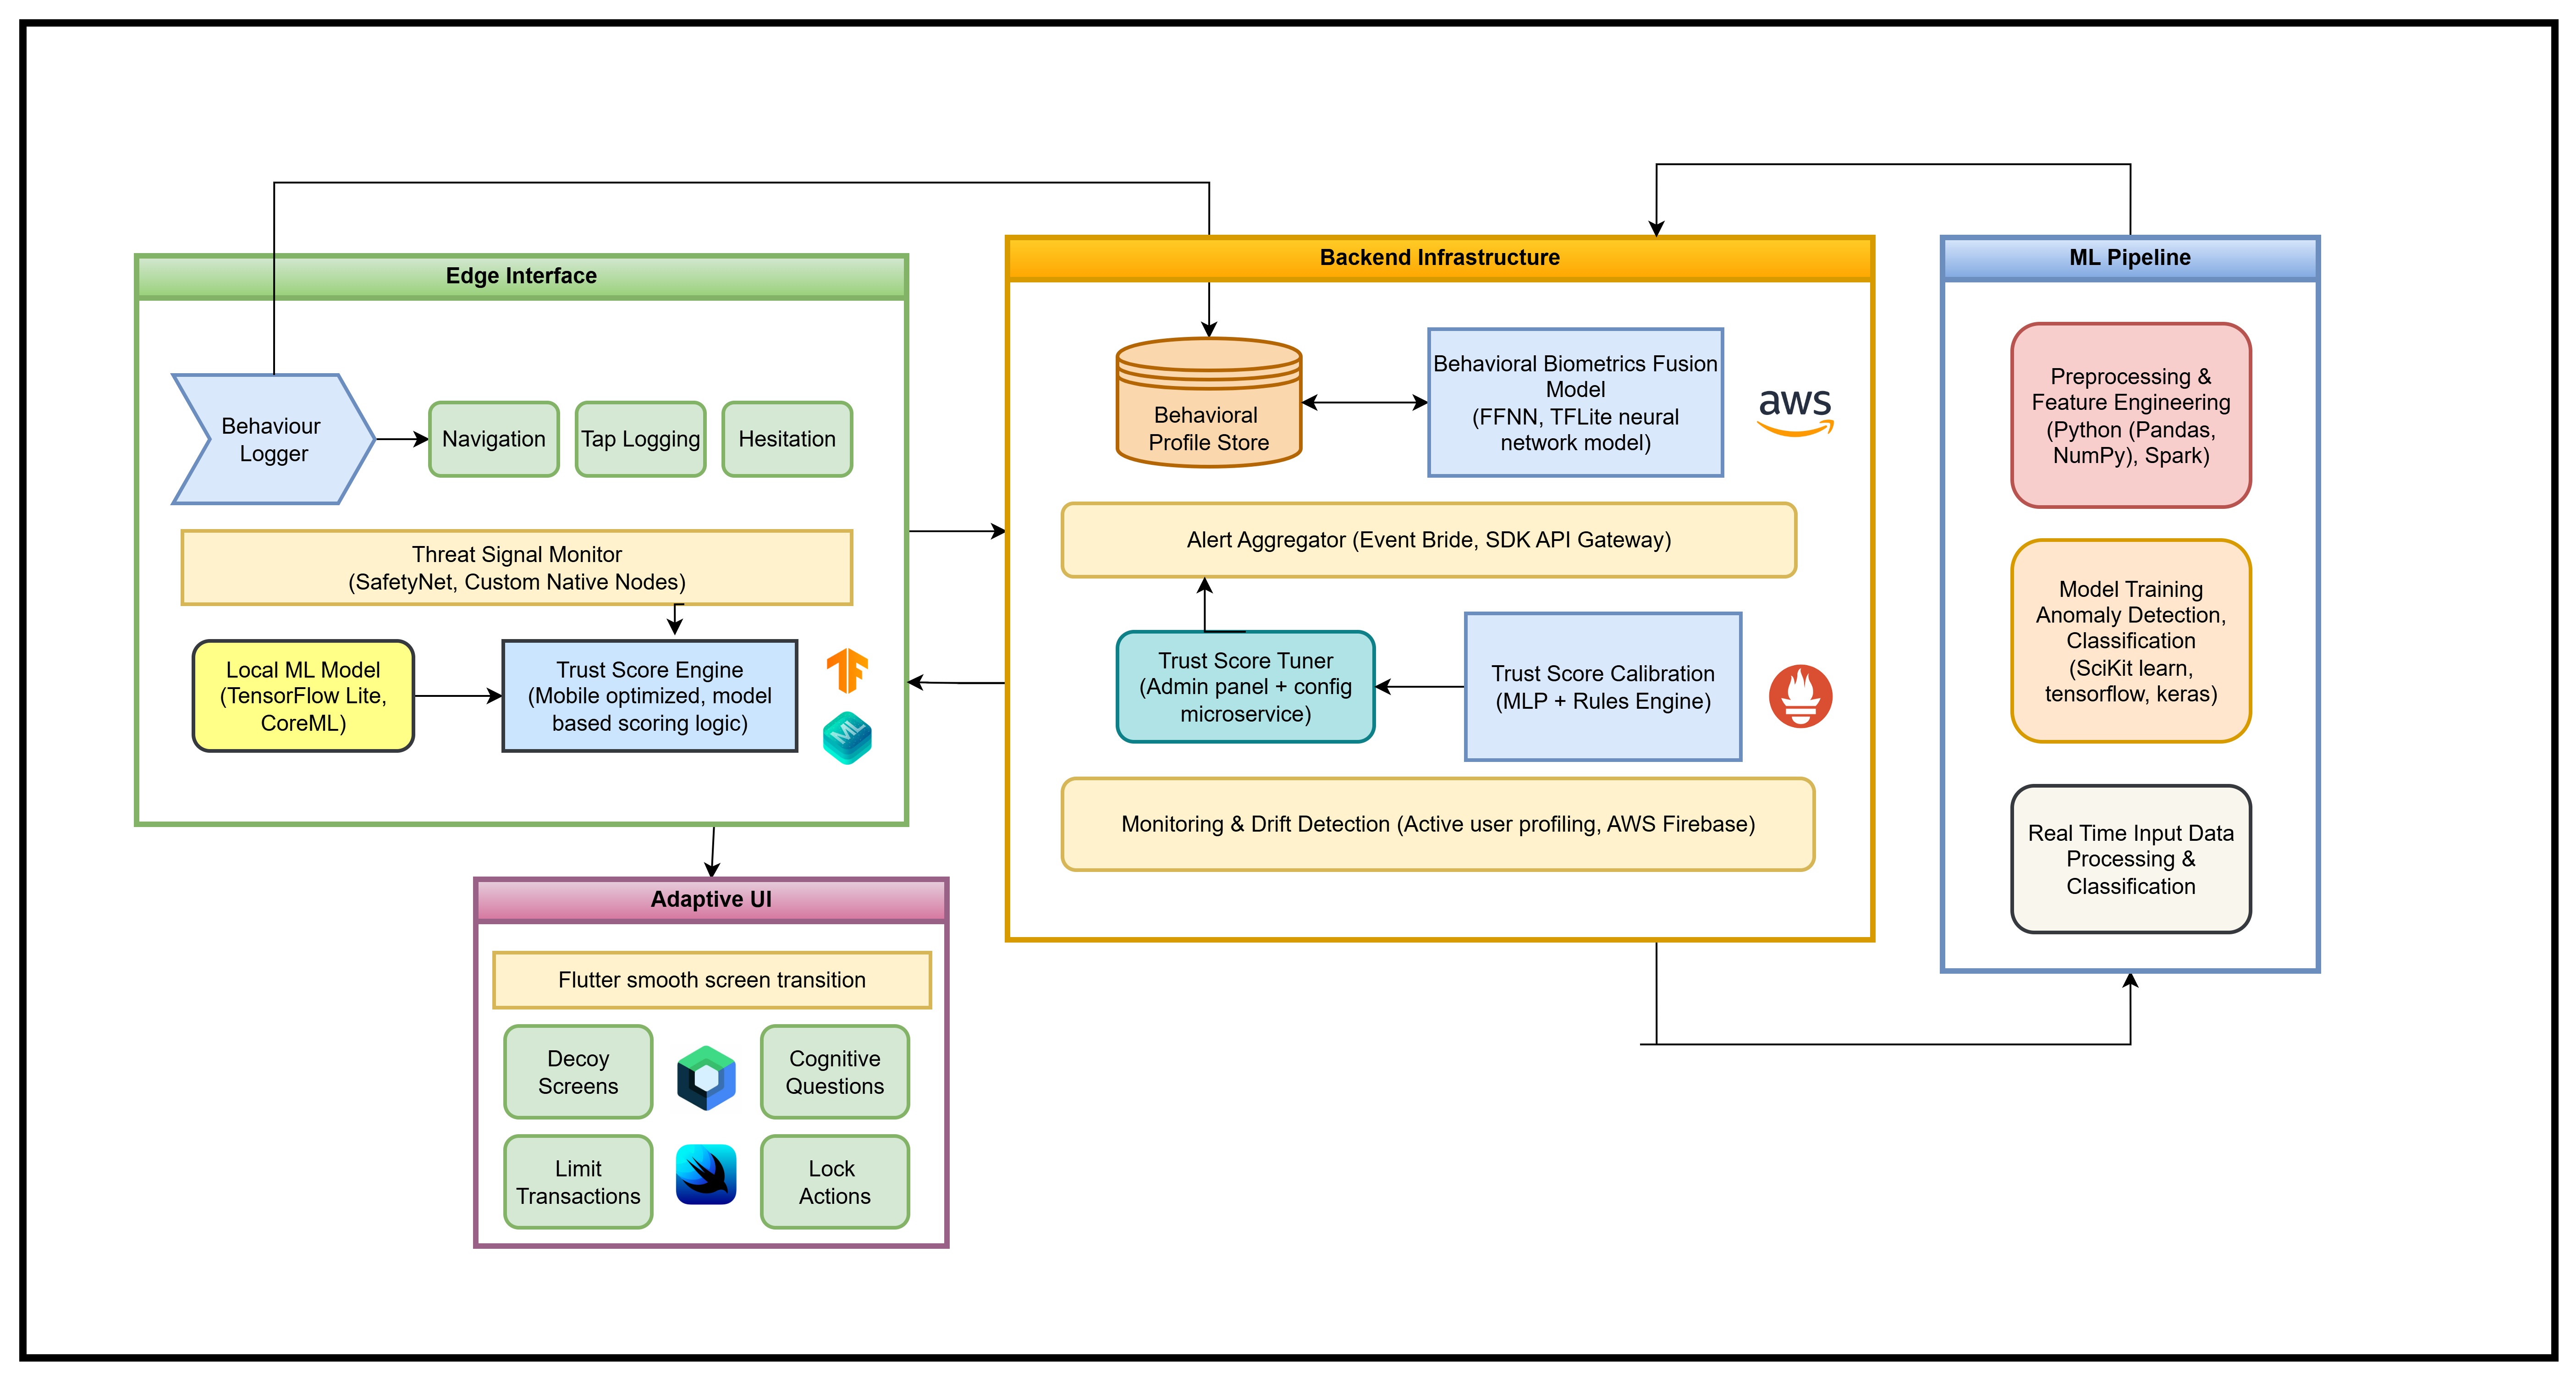
\includegraphics[width=\linewidth]{architecture.png}\\
        \vspace{0.5cm}
        
    }}
    \caption{PhishSafe SDK Architecture Overview}
    \label{fig:architecture}
\end{figure}

The PhishSafe SDK follows a modular architecture with these key components:

\begin{itemize}
    \item \textbf{Data Collection Layer}: Handles user interaction monitoring
    \item \textbf{Analysis Engine}: Processes behavioral patterns
    \item \textbf{Risk Assessment Module}: Calculates trust scores
    \item \textbf{Data Storage}: Manages session logs
\end{itemize}

\clearpage
\section{Implementation Guide}

\subsection{Basic Integration}

\subsubsection{Initialize the SDK}
Add initialization in your app's main entry point:

\begin{lstlisting}[language=Dart]
void main() async {
  WidgetsFlutterBinding.ensureInitialized();
  
  await PhishSafeSDK.configure(
    PhishSafeConfig(
      enableLocationTracking: true,
      logLevel: LogLevel.info,
    ),
  );
  
  runApp(MyApp());
}
\end{lstlisting}

\subsubsection{Session Management}
Wrap your authentication flow:

\begin{lstlisting}[language=Dart]
void loginUser() async {
  try {
    await PhishSafeSDK.initSession();
    // Proceed with login
  } catch (e) {
    // Handle error
  }
}

void logoutUser() {
  PhishSafeSDK.endSession();
  // Clear user session
}
\end{lstlisting}

\subsection{Module Integration Details}

\subsubsection{Main Interface – phishsafe\_sdk.dart\index{phishsafe\_sdk.dart}}
\textbf{What it does:} This file exposes all SDK functionalities to the external Flutter app, including session management, screen visit logging, and swipe/tap events.

\begin{lstlisting}[language=Dart]
import 'package:phishsafe_sdk/phishsafe_sdk.dart';

void main() async {
  WidgetsFlutterBinding.ensureInitialized();

  // Start PhishSafe SDK session
  PhishSafeSDK.initSession();

  runApp(MyApp());
}
\end{lstlisting}

\begin{lstlisting}[language=Dart]
// When session ends (e.g., user logs out)
await PhishSafeSDK.endSession();
\end{lstlisting}

Always call \texttt{initSession()} after successful authentication and \texttt{endSession()} when user explicitly logs out.

\subsubsection{Core Manager – PhishSafeTrackerManager\index{PhishSafeTrackerManager}}
\textbf{What it does:} Manages all trackers, detectors, and backend communication via a singleton.

\begin{lstlisting}[language=Dart]
final tracker = PhishSafeTrackerManager();
tracker.recordTapPosition(
  screenName: "HomePage",
  tapPosition: Offset(100, 150),
  tapZone: "center",
);
\end{lstlisting}

For most use cases, use the higher-level \texttt{PhishSafeSDK} interface instead of accessing the manager directly.

\subsubsection{RouteAwareWrapper\index{RouteAwareWrapper}}
\textbf{What it does:} Wraps screens to log visits and time spent.

\begin{lstlisting}[language=Dart]
final RouteObserver<PageRoute> routeObserver = RouteObserver<PageRoute>();

MaterialApp(
  navigatorObservers: [routeObserver],
  home: RouteAwareWrapper(
    screenName: "HomePage",
    observer: routeObserver,
    child: HomeScreen(),
  ),
);
\end{lstlisting}

Use consistent screen names across your app for accurate navigation pattern analysis.

\subsubsection{GestureWrapper\index{GestureWrapper}}
\textbf{What it does:} Captures taps and swipes with position and timing.

\begin{lstlisting}[language=Dart]
GestureWrapper(
  screenName: "TransferPage",
  child: Scaffold(
    body: Center(child: Text("Make a transfer")),
  ),
)
\end{lstlisting}

Wrap screens containing sensitive actions like money transfers for comprehensive gesture tracking.

\subsubsection{TapTracker\index{TapTracker}}
\textbf{What it does:} Tracks tap positions, zones, durations.

\begin{lstlisting}[language=Dart]
PhishSafeTrackerManager().recordTapPosition(
  screenName: "LoginPage",
  tapPosition: Offset(80, 120),
  tapZone: "top_left",
);
\end{lstlisting}

The SDK automatically tracks taps in wrapped widgets - manual recording is only needed for custom gesture handlers.

\subsubsection{SwipeTracker\index{SwipeTracker}}
\textbf{What it does:} Records swipe positions, speed, and duration.

\begin{lstlisting}[language=Dart]
PhishSafeTrackerManager().recordSwipeMetrics(
  screenName: "TransferPage",
  durationMs: 300,
  distance: 250.0,
  speed: 0.83,
);
\end{lstlisting}

Swipe velocity patterns are strong indicators of authentic vs. fraudulent behavior.

\subsubsection{InputTracker\index{InputTracker}}
\textbf{What it does:} Logs login, FD break, loan taken, transaction timing.

\begin{lstlisting}[language=Dart]
PhishSafeTrackerManager().recordFDBroken();
PhishSafeTrackerManager().recordLoanTaken();
PhishSafeTrackerManager().recordWithinBankTransferAmount("100000");
\end{lstlisting}

Call these methods immediately after financial transactions occur for most accurate timing data.

\subsubsection{LocationTracker\index{LocationTracker}}
\textbf{What it does:} Requests and returns geolocation.

\begin{lstlisting}[language=Dart]
Position? position = await LocationTracker().getCurrentLocation();
print("Latitude: ${position?.latitude}, Longitude: ${position?.longitude}");
\end{lstlisting}

Location tracking requires explicit user permission - handle permission requests gracefully.

\subsubsection{NavigationLogger\index{NavigationLogger}}
\textbf{What it does:} Logs screen visits with timestamps.

\begin{lstlisting}[language=Dart]
PhishSafeTrackerManager().onScreenVisited("LoanSummaryScreen");
\end{lstlisting}

For Flutter apps, prefer \texttt{RouteAwareWrapper} over manual screen visit logging.

\subsubsection{SessionTracker\index{SessionTracker}}
\textbf{What it does:} Tracks session start/end and duration.

\begin{lstlisting}[language=Dart]
PhishSafeTrackerManager().startSession();
// ...user actions...
await PhishSafeTrackerManager().endSessionAndExport();
\end{lstlisting}

Sessions automatically time out after 30 minutes of inactivity.

\subsubsection{ScreenRecordingDetector\index{ScreenRecordingDetector}}
\textbf{What it does:} Detects if screen recording is active.

\begin{lstlisting}[language=Dart]
final isRecording = await ScreenRecordingDetector().isScreenRecording();

if (isRecording) {
  print("WARNING: Screen recording is active!");
}
\end{lstlisting}

Consider showing a warning to users when screen recording is detected during sensitive operations.

\subsubsection{DeviceInfoLogger\index{DeviceInfoLogger}}
\textbf{What it does:} Gets platform, model, brand info.

\begin{lstlisting}[language=Dart]
final info = await DeviceInfoLogger().getDeviceInfo();
info.forEach((k, v) => print("$k -> $v"));
\end{lstlisting}

Device fingerprinting helps detect suspicious device changes between sessions.

\subsubsection{LocalStorage\index{LocalStorage}}
\textbf{What it does:} Simple key-value storage using SharedPreferences.

\begin{lstlisting}[language=Dart]
final storage = LocalStorage();

await storage.saveString("user_id", "user123");
final userId = await storage.readString("user_id");
await storage.deleteKey("user_id");
\end{lstlisting}

Use for temporary session data - not for sensitive information.

\subsubsection{ExportManager\index{ExportManager}}
\textbf{What it does:} Exports session logs to local + cloud.

\begin{lstlisting}[language=Dart]
final manager = ExportManager();
final dummySession = {
  "session": {"start": "2025-07-27T10:00:00Z", "end": "2025-07-27T10:10:00Z"},
  "tap_events": [],
};

await manager.exportToJson(dummySession, "session_log");
\end{lstlisting}

Default Log Storage Location
Exported logs are stored in \texttt{/sdcard/Download/PhishSafe/} by default.

\subsubsection{ApiService\index{ApiService}}
\textbf{What it does:} Sends events to the backend Flask API.

\begin{lstlisting}[language=Dart]
await ApiService.sendTapEvent(
  screenName: "Dashboard",
  position: Offset(150, 200),
  tapZone: "bottom_right",
);
\end{lstlisting}

\begin{lstlisting}[language=Dart]
await ApiService.sendScreenVisit("LoginPage");
await ApiService.sendSessionEnd(DateTime.now());
\end{lstlisting}

The SDK handles API communication automatically - manual calls are rarely needed.

\subsubsection{Full Integration Sample\index{Full Integration Sample}}

\begin{lstlisting}[language=Dart]
final RouteObserver<PageRoute> observer = RouteObserver<PageRoute>();

MaterialApp(
  navigatorObservers: [observer],
  home: RouteAwareWrapper(
    observer: observer,
    screenName: "LoginScreen",
    child: GestureWrapper(
      screenName: "LoginScreen",
      child: LoginScreen(),
    ),
  ),
);
\end{lstlisting}

This comprehensive wrapping provides the most complete behavioral data collection.


\clearpage
\section{Data Storage}
All session logs are saved in JSON format at:
\begin{lstlisting}
/sdcard/Download/PhishSafe/
\end{lstlisting}

Sample log structure:
\begin{lstlisting}[language=json]
{
  "session_id": "abc123",
  "start_time": "2025-07-20T10:00:00Z",
  "device_info": {
    "model": "Pixel 6",
    "os": "Android 14"
  },
  "trust_score": 85,
  "anomalies": []
}
\end{lstlisting}

\clearpage

\end{document}